\begin{figure*}[t]
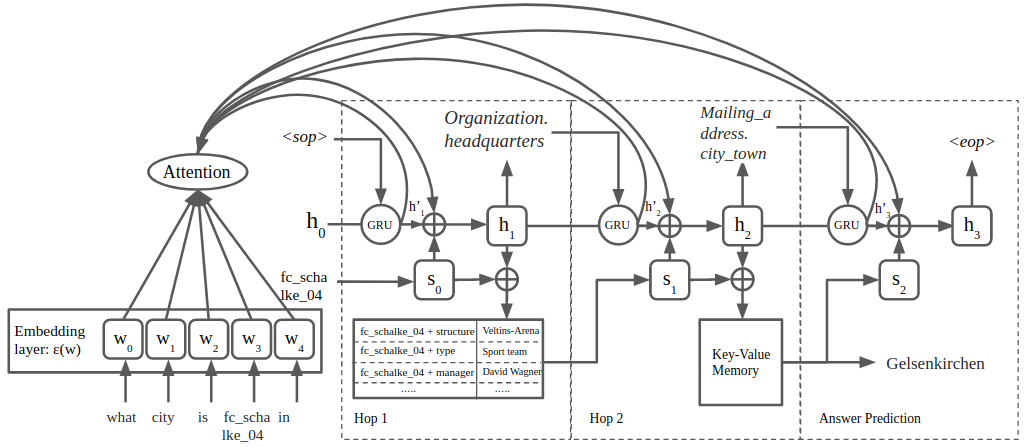
\includegraphics[width=2.1\columnwidth]{figs/model2.png}
\caption{\fontsize{10}{12}\selectfont An illustration of how our model answers the question "What city is fc\_schalke\_04 in?". The entity linker extracts \textit{fc\_schalke\_04} as the topic entity. $[\textit{\textless sop\textgreater}, \textit{Organization.headquarters} , \textit{Mailing\_address.city\_town, \textless eop\textgreater}]$ is the predicted relation path \cheng{Shall we include entities in the middle in the path? Are sop and eop defined already?} and \textit{Gelesenkirchen} is the predicted answer. The symbol $\bigoplus$ represents concatenation. }
\label{fig:model}
\end{figure*}


\section{Model}
 Given a question $q$ and its topic entity $e_0$ (identified by entity linking \cheng{Did we mention entity linking before?}), our model aims to find the reasoning path $\mathbf{p} = (e_{0},r_{1},e_{1},r_{2}, \cdots,e_{T-1}, r_{T})$ and the answer $y$ from the knowledge base $\mathcal{KB}$. In this section, we first present the design of our model architecture, and then explain the training and inference algorithms in detail.  

\subsection{Model Architecture}


Figure \ref{fig:model} illustrates the architecture of our model. Our base model is similar to a RNN structure.

 All the words $w_0,w_1,\cdots,w_{|q|-1}$ in the given question $q$ are first sent to a fixed embedding layer to acquire word embeddings $\varepsilon_w(w_0),\varepsilon_w(w_1),\cdots,\varepsilon_w(w_{|q|-1})$. \cheng{Does the symbol match the one in diagram?} To reduce computational cost, the embedding layer is pre-trained and not updated during RNN training. Because we wish to learn different question context representations to show different reasoning focus at each hop, the  word embeddings are combined in different ways to form the question embedding  based on attention weights learned by relation prediction module at each hop.
% $\varepsilon(\cdot)$ function represents gathering embedding of the input from the corresponding pre-trained embeddings matrix. 



%\subsubsection{Reasoning Decoding} The decoding module consists of relation prediction module and entity prediction module.


We model relation prediction as a sequence prediction task using recurrent neural network with gated recurrent units (GRU). The hidden representations of GRU unit and predicted relation at timestep $t$ are denoted by $h_t$ and $r_t$ respectively. At timestep $t$, the model relies on the attention mechanism~\cite{DBLP:journals/corr/BahdanauCB14} to produce a question context vector $c_t$. Specifically we first apply GRU to produce a temporary hidden state  $h_{t}'=GRU(h_{t-1}, r_{t-1})$, and then apply a parameterized feed-forward neural network $a$ to calculate the similarity score $u_{tk} = a(h'_{t},\varepsilon_w(w_k))$ of two inputs $h'_{t}$ and $\varepsilon_w(w_k)$,  and then these scores are normalized into attention weights $\alpha_{tk}=\frac{\exp (u_{tk})}{\sum_{0\leq j\leq |q|-1}\exp (u_{tj})}$, which are used to produce the question context vector $c_t=\sum_{0\leq j\leq |q|-1}\alpha_{tj}\varepsilon_w(w_j)$. 
% \begin{align}
% h'_{t} = GRU(h_{t-1}, r_{t-1}) 
% \end{align}
% \vspace{-3ex}
% \begin{align}
% u_{tk} = a(h'_{t},\varepsilon(w_k))
% \end{align}
% \vspace{-3ex}
% \begin{align}
% \alpha_{tk} = \frac{\exp (u_{tk})}{\sum_{0\leq j\leq |q|-1}\exp (u_{tj})}
% \end{align}
% \vspace{-1ex}
% %\[\alpha_{tk} = \frac{u_{tk}}{\sum_{j}u_{tj}}\]
% \begin{align}
% c_t = \sum_{0\leq j\leq |q|-1}\alpha_{tj}\varepsilon(w_j)
% \end{align}

 %After having all above computations done, 

The model then concatenates temporary hidden state $h_{t}'$, entity representation $\varepsilon_e(e_{t-1})$, and question context $c_t$ together, and pass the concatenation through a linear transformation $f$ with ReLU activation to obtain the hidden state $h_t=ReLU(f([h'_{t}; \varepsilon_e(e_{t-1}); c_t]))$. 

\subsection{Probabilities and Objective Function} 
The probability of predicting the $k$-th relation $\gamma_k$ in $\mathcal{R}$ at timestep $t$ is 
\begin{align*}
&P(r_t=\gamma_k|q,e_0,r_1,\cdots,e_{t-1})\\
 &= \frac{\exp <h_t,\varepsilon_r(\gamma_k)>}{\sum_j\exp <h_t,\varepsilon_r(\gamma_j)>}=o^k_t,
\end{align*}
where $\varepsilon_r$ is the embedding function, $<>$ is the dot product between two inputs 


Given the previous entity $e_{t-1}$ and relation $r_t$, the next matched entity may not be unique when we query the knowledge base (another way to collect this entity is via a soft lookup with a key-value memory network structure. We provide more details in the appendix.)  For example, if $e_{t-1}$=``united states'', and $r_t=$ ``president of'', then the resulting entity has 45 possibilities. Without additional constraints, all of them are equally likely to be selected, and hence we define 
\begin{align*}
        &p(e_t|e_0,r_1,\cdots,e_{t-1},r_t,q)\\
        =&p(e_t|e_{t-1},r_t)\\
        =&\begin{cases}
        1/M & \text{if }e_t\text{ is one of the }M\text{  matched entities} \\
        0 & \text{if }e_t\text{ is not a matched entity}
\end{cases}    
\end{align*}

We assume that there are multiple valid paths $\mathbf{p}$ that can lead to the correct answer $y$ and they are not given by the annotator in the dataset. We treat these paths as hidden variables and we marginalize them out to compute the probability of getting the answer $y$.
\kechen{remove P(e0 given q)? and define $\mathcal{P}$?}
\begin{align}
&p(y|q)\nonumber\\
=&\sum_{\mathbf{p}\in\mathcal{P}} p(y|\mathbf{p},q)p(\mathbf{p}|q)   \nonumber\\
=&\sum_{\mathbf{p}\in\mathcal{P}}\{p(y|e_{T-1},r_T)p(e_0|q)\prod_{t=1}^{T-1} p(e_t|e_{t-1},r_t)\nonumber\\ &\prod_{t=1}^T p(r_t|q,e_0,r_1,\cdots,e_{t-1})\}
\label{eq:marginal}
\end{align}
\kechen{P(stop)}

To train our model, we would like to maximize the answer probability $p(y|q)$ using only the given answer for each training instance. To make prediction on each test case, we would like to find the answer $y$ with the highest probability.

The way we define answer probability as in Eq.~(\ref{eq:marginal}) is  novel in the KBQA task. Most of the existing methods assume the availability of a single ground truth path annotation and aim to maximize the probability of the given path~\cite{DBLP:conf/coling/ZhouHZ18}. As we will demonstrate later in the result section, considering multiple paths leads to better model performance.









%To further improve the diversity of the outputs, we follow \newcite{}'s idea to optimize mutual information instead of log likelihood. Specifically, we observe that 


\subsection{Training}
\kechen{merge 2.2 to 2.1.3 and create new 2.2 only for training algorithm? should we keep join objective here?}

Training this objective requires summing up all valid relation paths from the topic entity to the answer entity in the knowledge base. Thus evaluating this objective exactly can be intractable. As we showed in the early example, some relation paths ($R_5, R_6, R_7$ in Figure \ref{QAPaths}) are not very helpful to training \kechen{P(y|R567) is very small in the marginalization}, and thus should be removed from training or assigned low probabilities. To achieve this goal, we first apply depth first search (DFS) algorithm with maximize 3 hops to get valid path candidates. The algorithm starts traversal from the topic entity node and ends at the answer entity node. All possible paths between the topic entity and the answer entity within 3 hops are extracted as candidates. We then set a threshold to remove paths which point to too many entities at the last hop. To further filter out bad relation paths, we propose to dynamically choose relation paths deemed as most probable by the current model during training.


 The overall training procedure is summarized in Algorithm \ref{alg:train}. Note that training with this algorithm does not require ground truth relation path label. Labeled relation path can be seen as plus, but not necessary. If it is given, we can either replace $\mathcal{P}$ with ground truth relation set, or train the model with joint probability objective using ground truth label first and transit to marginal probability objective after a few epochs.

\begin{algorithm}
  \SetKwInOut{Input}{Input}
  \SetKwInOut{Output}{Output}

 % \underline{function Euclid} $(a,b)$\;
  \Input{KBQA dataset $(q^{(n)},y^{(n)}, e_0^{(n)}),n=1,2,\cdots,N$, \\
  Knowledge Base $\mathcal{KB}$, \\
  Threshold $k_1$ and $k_2$. }
  \Output{Trained model parameters}
  Use DFS algorithm to get a set of paths $\mathcal{P}$ from $e_0^{(n)}$ to $y^{(n)}$.\\
  Remove paths that point to more than $k_1$ entities from $\mathcal{P}$.\\
  % Initialize model parameters\\
  \ForEach {batch}{
    % \ForEach {batch }{
      \ForEach{$(x^{n},\mathbf{y}^{n})$ in the batch}{
        Get top $k_2$ paths of $\mathcal{P}$ sorted by $P(\mathbf{p}|q)$ :\\
		  	$\{{\mathbf{p}}^n_{1},\cdots,{\mathbf{p}}^n_{k_2}, P({\mathbf{p}}^n_{1}|q^n),\cdots,P({\mathbf{p}}^n_{K}|q^n,$ $P({y}^n_{1}|{\mathbf{p}}^n_{1},q^n),\cdots,P({y}^n_{K}|{\mathbf{p}}^n_{n},q^n)\}$ \hspace{4ex}= Inference\_with\_current\_model$(q^{n},\mathcal{P}$)\\
		  	$\mathcal{P} = \{{\mathbf{p}}^n_{1},\cdots,{\mathbf{p}}^n_{k_2} \}$\\
        }  
              Update model parameters by maximizing $\sum\limits_{(q^{n},{y}^{n}) \in \text{batch}} \log \sum\limits_{\mathbf{p} \in \mathcal{P}}  P(y^{n}|\mathbf{p},q^{n}) P(\mathbf{p}|q^{n}) $
        }


    % }
  \caption{Training method}
  \label{alg:train}
\end{algorithm}
\subsection{Inference} \kechen{emphasize beam search is only a way to collect probabilities rather than the real prediction method}


We adopt beam search to predict the relation path and use knowledge base lookup to predict the answer. Different from the vanilla beam search that allows to search on the full set of relations $\mathcal{R}$. We add two constraints to beam search so as to only select the valid path based on the knowledge base. (1) The first relation should get connected with the topic entity. (2) Each relation should get connected with the previous relation where uses an entity as the bridge. We then use an ensemble strategy to re-rank the searching results. Formally, given beam search outputs $\mathbf{p}_{1},\cdots,\mathbf{p}_{b}$ and $P(\mathbf{p}_{1}),\cdots,P(\mathbf{p}_{b})$, our model first use knowledge base lookup to get a list of different answer sets $\hat{y}_1,\cdots,\hat{y}_m$, where $m$ is the number of answer sets generated by $b$ relation paths, hence $m \leq b$. We then take the sum of the probabilities of relation paths $\mathbf{p}_i$ leading to the same predicted answer set and compare these sums. The final selected answer set $\hat{y}$ is the one with the maximum sum value. To represent it mathematically:
\begin{equation}
\hat{y}=\argmax_{\hat{y}_l} \sum_{i} P(\mathbf{p}_i\rightarrow \hat{y}_l)
\end{equation}
where $P(\mathbf{p}_i\rightarrow \hat{y}_l)$ is the probability of a relation path leading to the predicted answer set $\hat{y}_l$ and $l \in \lbrace 1, \cdots, m\rbrace$. 

\begin{equation}
\begin{aligned}
&\log PMI(y;f^{-ent}|f^{ent})\\
=& \log\frac{P(y,f^{-ent}|f^{ent})}{P(y|f^{ent})P(f^{-ent}|f^{ent})}\\
=& \log\frac{P(y|f^{-ent},f^{ent})}{P(y|f^{ent})}\\
=& \log P(y|f^{-ent},f^{ent})-\log P(y|f^{ent})\\
=& \log\sum_{\mathbf{p}\in\mathcal{P}}P(y,\mathbf{p}|f^{-ent},f^{ent}) - \log\sum_{\mathbf{p}\in\mathcal{P}}P(y,\mathbf{p}|f^{ent})\\
\end{aligned}
\end{equation}

where $f^{-ent}$ represent all info without using entity\kechen{unify $P(x),p(x)$}

\kechen{mutual info}
